\documentclass{simpledoc}

\newcommand{\mgpost}{\texttt{mgpost}\ }
\newcommand{\yade}{\texttt{yade}\ }
\newcommand{\var}[1]{$<$#1$>$}
\newcommand{\opt}[1]{$[$#1$]$}
\newcommand{\file}[1]{\textit{#1}}
\newcommand{\screen}[1]{\texttt{#1}}
\newcommand{\key}[1]{\fbox{#1}}


\title{mgpost -- A quick user guide}
\author{Vincent Richefeu\\
vincent.richefeu@hmg.inpg.fr\\
Laboratoire 3S-R\\
Grenoble, France\\
}

\pagestyle{myfootings}
\markboth{mgpost: user guide}%
         {mgpost: user guide}

%%%%%%%%%%%%%%%%%%%%%%%%%%%%%%%%%%%
%%%%%%%%%%%%%%%%%%%%%%%%%%%%%%%%%%%
\begin{document}

\maketitle

\begin{abstract}
This document describes (very shortly) how to use the soft \mgpost dedicated to 
post-processing and 2D/3D visualization of discrete numerical simulations.
\end{abstract}

\tableofcontents

\newpage

\section{Introduction}

\mgpost is a small soft for viewing 
2D or 3D discrete element simulations. These simulations can be 
performed with the computer code of your choice.
The interface between the computer code and \mgpost is performed through MGP files.
It is actually a XML format\footnote{http://www.w3c.org} similar to the HTML format, with 
specific tags. This format will be described thereafter.

\mgpost uses the OpenGL API standard 
for 2D and 3D vectorial graphics. It can currently be 
be compiled on the Linux operating system, Windows or Mac OS X.
%
\begin{figure}[H]
\begin{center}
\ifpdf
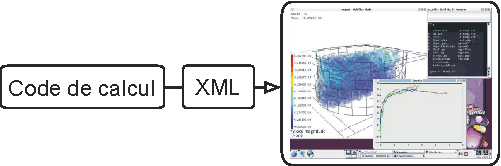
\includegraphics[width=11cm]{figs/xml.png}
\else
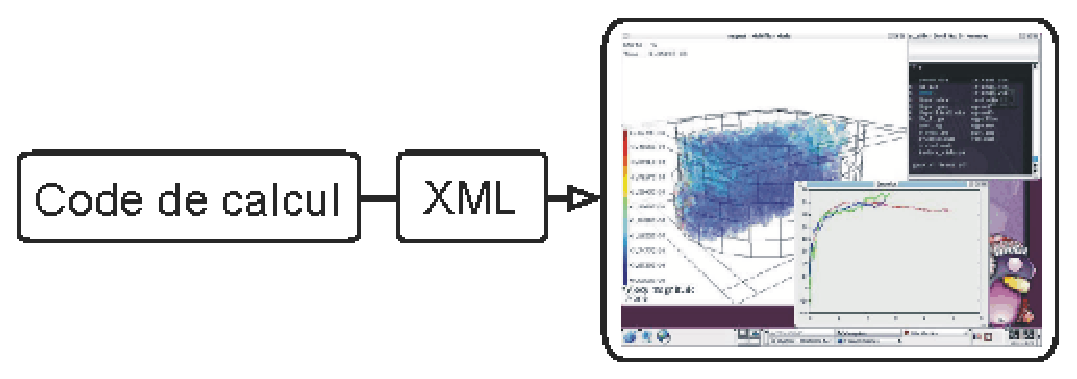
\includegraphics[width=11cm]{figs/xml.eps}
\fi
\end{center}
\caption{\emph{XML format that interface the computational code with } \mgpost}
\label{fig:xml_interface}
\end{figure}

\attention
By distributing this soft freely, the objective is to facilitate the 
post-processing and visualization of 2D/3D academic simulations 
by the discrete element methods. We thank you for your possible comments and ask you to refer to 
the soft \mgpost as a part of yade if you use it for a publication or communication.

\subsection{Notations used}

The document uses the conventions listed below:

\begin{itemize}

\item \screen{text that appear on the screen (Tele Type)}

\item \key{key}

\item \file{file name}

\item \textnormal{text of the document (Times)}

\item \var{var} : variable (to replace by a value)

\item \opt{opt} : optional information

\item Symbol \$ : prompt

\end{itemize}

\section {Running \mgpost}

\subsection {Parameters}

\mgpost can be launched with the following parameters:

\marginlabel{\texttt{-v}} 
Display the current version of \mgpost.

\begin{verbatim}
  $ mgpost -v

       mgpost version 0.5.3, V. Richefeu
       mgpost comes with ABSOLUTELY NO WARRANTY.
\end{verbatim}

\marginlabel{-files} 
Create the files \file{mgpalloc} and \file{mgconf}.

% \begin{verbatim}
%   $ mgpost -files
%     File 'mgpalloc' created
%     File 'mgconf' created
% \end{verbatim}

\marginlabel{\texttt{-mgpalloc}} 
Create the file \file{mgpalloc}.

\begin{verbatim}
  $ mgpost -mgpalloc
    File 'mgpalloc' created
\end{verbatim}

\marginlabel{\texttt{-mgconf}}
Create the file \file{mgconf}.

\begin{verbatim}
  $ mgpost -mgconf
    File 'mgconf' created
\end{verbatim}

\marginlabel{\texttt{-i \var{filename}}} 
Read the file named filename.

\begin{verbatim}
  $ mgpost -i MySimulation.mgp
\end{verbatim}

\marginlabel{\texttt{-mf \opt{\var{state number}}}}
Reading a series of MGP files named \file{mgp.out.\textbf {nnn}}  
in the current directory. If the number of the state is not 
given, the option -mf must be the last in the list; state number default value is 1.

\begin{verbatim}
  $ mgpost -mf 50
\end{verbatim}

\marginlabel{\texttt{-mfz \opt{\var{state number}}}}
Reading a series of MGP files named \file{mgp.out.\textbf {nnn}.gz}  
in the current directory. If the number of the state is not 
given, the option -mf must be the last in the list; state number default value is 1.

\begin{verbatim}
  $ gzip -9 mgp.out.*
  $ mgpost -mfz
\end{verbatim}

\marginlabel{\texttt{-r0}}
Visualize the sample without center it on the global framework.

\begin{verbatim}
  $ mgpost -i MySimulation.mgp -r0
\end{verbatim}

\marginlabel{\texttt{-dim \var{width} \var{height}}}
Define the window dimensions.

\begin{verbatim}
  $ mgpost -i MySimulation.mgp -dim 500 600
\end{verbatim}

\marginlabel{\texttt{-2d}}
Force \mgpost to set the mode 2D (by default, the mode 3D is chosen). The mode can be changed at run-time by pressing the touch 2 or 3 of the keyboard.

\begin{verbatim}
  $ mgpost -i MySimulation.mgp -2d
\end{verbatim}

\marginlabel{\texttt{-mono}}
Force \mgpost to use a gray level color scale (it cannot be modified at run-time).

\begin{verbatim}
  $ mgpost -i MySimulation.mgp -mono
\end{verbatim}

\marginlabel{\texttt{-section \var{a} \var{b} \var{c} \var{d}}}
Define the parameters  $a$ $b$ $c$ and $d$ of the plan given by:

\begin{equation}
aX + bY + cZ + d = 0 
\end{equation}

This plan allows us to realize sections through 3D samples.
The vector $(a\;b\;c)^T$ correspond to the normal and 
 $d$ is the distance from the origine (of the  framework).
$d$ can be modified at run-time with the 'up' and 'down' arrow keys.

\begin{verbatim}
  $ mgpost -i MySimulation.mgp -section 1 0 0 0
\end{verbatim}

\marginlabel{\texttt{-dsec \var{distance}}}
Define half the width of a section.

\begin{verbatim}
  $ mgpost -i MySimulation.mgp -dsec 5.0e-3
\end{verbatim}

\subsection{Multi-files and Mono-file modes}

Mono-file mode is activated when with the option \screen{-i \var{\file{filename.mgp}\opt{.gz}}}.
Multi-files mode is activated with the option -mf or -mfz (files \file{mgp.out.\textit{nnn}\opt{.gz}}).

For both Mono- and Multi-files modes, navigation between the stored states can be made with the keys \key{+} and \key{-}. The key \key{0} is to Show the first state (corresponding to the file \screen{001} with Multi-files mode).

\attention
The MGP files must be placed into the current folder (\screen{pwd}).

\section{IHM}

\subsection{Mouse usage}

\marginlabel{left button kept pressed and move} Rotate the sample

\marginlabel{middle button kept pressed and move} Zoom. 

\marginlabel{right button} Menu.

\marginlabel{CTRL + left button} Select a body. 
When a body is selected, press the key \key{i} to obtain
information about the selected body only.

\subsection{Some usefull shortcuts}

\marginlabel{\key{space}}
Stop playing the simulation.

\marginlabel{\key{c}}
Swap the affectation of the color scale between bodies and interactions.

\marginlabel{\key{d}}
Display body shapes.

\marginlabel{\key{e}}
Display (only) the bounding box of the sample.
This is usefull when there is to much bodies. displaying is thus very faster.

\marginlabel{\key{h}}
Display on the terminal a quick help.

\marginlabel{\key{i}}
Display on the terminal some informations on the sample if no body is selected, and on the selected body otherwise.

\marginlabel{\key{n}}
Display the bidy numbers.

\marginlabel{\key{o}}
Display body orientations.

\marginlabel{\key{p}}
Display the center positions of the bodies.

\marginlabel{\key{q}}
Quit \mgpost.

\marginlabel{\key{r}}
Display the global framework  (on/off).

\marginlabel{\key{s}}
Smooth the bodies (slow) for screenshots.

\marginlabel{\key{t}}
Display the current time (on/off).

\marginlabel{\key{w}}
Run a 'movie' of the stored states.

\marginlabel{\key{z}}
Display only the controled bodies (with \screen{isDynamics = false} in YADE).

\marginlabel{\key{/}}
Cut (plan parallel to the screen) the sample at coordinate (0, 0, 0).

\marginlabel{\key{*}}
cancel the cutting with key \key{/}.

\marginlabel{\key{0}}
Come again to the first stored state.

\marginlabel{\key{2}}
Mode 2D.

\marginlabel{\key{3}}
Mode 3D.

\section {Input files}

There is 3 types of input files: \file{mgconf} and \file{mgpalloc} that make it possible to define parameters, and MGP files that contain the data from the simulation.

\subsection{\screen{mgconf} file}
        
This file set the major options for graphic display. It is simply a
text file that contains keywords followed by one or more values.
Both keywords and values are 'tokens'. They are separated by characters of your choice among the following:
space, equal, tab, comma, semi-colon, parentheses, accolades.
The file is interpreted by \mgpost line by line.
The values associated with a keyword must be on the same line.
Everything that follows the character \textbf{\#} ou \textbf{!} is ignored to put comments in the file.

\subsubsection{Example}

\begin{lstlisting}[style=mgpdata]
# Window size
W = 500 ; H = 500 

# couleurs
funRGB = (0.5, 0.5, 0.8)
bgcolor  = fun 
fgcolor  = blue
fgcolor1 = black
fgcolor2 = red

# To draw a grid into the sample
GridXYZ = (1.0e-2 , 1.0e-2 , 1.0e-2)

# color levels
autoScaleColors = yes
max = 1.0e0  ! correspond to red
min = -1.0e0 ! correspond to blue
\end{lstlisting}

\subsubsection{Description of the file}

\marginlabel{W}
Width of the window (interger).

\marginlabel{H}
Heigth of the window (integer).

\marginlabel{funRGB}
rvb components (between 0.0 and 1.0) for a custom color.
Some colors already exist in \mgpost. They are \screen{blue}, \screen{white} 
\screen{green}, \screen{black}, \screen{yellow} and \screen{red}.
 
\marginlabel{bgcolor}
Background color.

\marginlabel{fgcolor}
Main foreground color (text, body shapes...)

\marginlabel{fgcolor1, fgcolor2}
Other foreground colors.

\marginlabel{GridXYZ}
Distances X, Y and Z to draw a squared grid into the sample.

\marginlabel{autoScaleColors}
Flag that indicate if the maximum and minimum values are fixed or not.
if \texttt{autoScaleColors = no} then the limit values are \screen{max} and \screen{min}.


\subsection{\screen{mgpalloc} file}

This file 'says' \mgpost to allocate enough memory space to allow visualization of various bodies and associated informations.

\subsubsection{Example}

\begin{lstlisting}[style=mgpdata]
  nb_times                  200
  nb_bodies                 2000
  nb_interactions_per_body  12
  nb_data_per_body          1
\end{lstlisting}

\subsubsection{Description}

\marginlabel{nb\_times}
Number of states per MGP file. 

\marginlabel{nb\_bodies}
Number of bodies per MGP file.

\marginlabel{nb\_interactions\_per\_body}
Maximum number of interactions per body and per state.

\marginlabel{nb\_data\_per\_body}
Maximum number of supplementary data per body. This data are usually used to describe complex geometries (eg. nodes and faces of polyedres, axis of Sweep Sphere Line Segments)

\subsection{Files *.mgp or mgp.out.\textit{nnn}}

These files contain the data needed to
visualization of various bodies with their associated data

\subsubsection{MGP file(s)}

A MGP file is a XML (eXtensible Markup Language) document. in other word, it is a text file that can be 'seen' with a simple text editor.
The file is composed of store spaces named \textit{entities} that contain other entities or parameters.\\ 

The general structure is as follows:\\

\begin{itemize}

\item a markup entity 'saying' that this is a XML document.

\begin{lstlisting}[style=mgpdata]
  <?xml version="1.0"?>
\end{lstlisting}

\item The root entity \screen{mgpost} (level 0). The parameter \screen{mode} (2D or 3D) can be set.

\begin{lstlisting}[style=mgpdata]
  <mgpost mode="2D">
    ...
  </mgpost>
\end{lstlisting}

\item One or more entities \screen{state} (level 1) corresponding to a given time during the simulation.

\begin{lstlisting}[style=mgpdata]
  <mgpost mode="2D">
    <state time="0">
      ...
    </state>
    <state time="0.1">
      ...
    </state>
    ...
  </mgpost>
\end{lstlisting}

\item The entities \texttt{body} (level 2) describing the body data.

\begin{lstlisting}[style=mgpdata]
  <mgpost mode="2D">
    <state time="0">
      <body>
          ...
      </body>
      <body>
          ...
      </body>
      ...
    </state>
    ...
  </mgpost>
\end{lstlisting}

\end{itemize}

Within the entity  \screen{body} one (and only one) shape is defined followed by the interaction data.

\begin{lstlisting}[style=mgpdata]
      <body>
        <DISKx>
          <position x="0" y="1"/>
        </DISKx>
        <DKDKx j="2" rn="0" rt="0">
        <DKDKx j="3" rn="1.254e-4" rt="0">
      </body>
\end{lstlisting}

\subsubsection{Body shape entities}

\marginlabel{DISKx}

\begin{lstlisting}[style=mgpdata]
  <DISKx r="0.004">
      <position x="0" y="0" rot="0.000031"/>
      <velocity x="-0.000076" y="-0.000133"/>
  </DISKx>
\end{lstlisting}

\marginlabel{SPHER}

\begin{lstlisting}[style=mgpdata]
  <SPHER r="0.002182">
     <position x="0" y="0.011137" z="0.016"/>
     <velocity x="0" y="-0.058855" z="0"/>
  </SPHER>
\end{lstlisting}

% \marginlabel{JONCx}
% On doit indiquer en attribut les longueurs \texttt{ax1} et
% \texttt{ax2}. Pour plus d'informations sur cette forme, voir la
% documentation du code de calcul LMGC90.
% 
% \begin{lstlisting}[style=mgpdata]
%   <JONCx ax1="0.048" ax2="0.002">
%     <position x="0.24e-01" y="0.24641e-01" rot="0.3141592e+01"/>
%     <velocity x="0" y="-0.1e-03" z="0"/>
%   </JONCx>
% \end{lstlisting}

\marginlabel{WALLX, WALLY ou WALLZ}

\begin{lstlisting}[style=mgpdata]
  <WALLX pos="-0.015"/>
  <WALLX pos="0.3"/>
  <WALLY pos="-0.015"/>
  <WALLY pos="0.3"/>
  <WALLZ pos="-0.015"/>
  <WALLZ pos="0.3"/>
\end{lstlisting}


%\marginlabel{MBRxx} \textit{TODO}

%\marginlabel{SEGMT} \textit{TODO}

%\marginlabel{CYLYx} \textit{TODO}

\marginlabel{POLYG} \textit{TODO}

\marginlabel{POLYE} \textit{TODO}

\subsubsection{Body data} \label{sec:marq_donnees}



\marginlabel{position} 

\begin{lstlisting}[style=mgpdata]
  <position x="0.000000" y="0.011137" z="0.016000"/> 
\end{lstlisting}

\attention
the Y axis is vertical.

\marginlabel{node}
Node coordinates of a polyhedra or a polygon. The
nodes are numbered from 0 in the order they appear
in the file. In the case of polygons, the nodes must be
described in the trigonometric order.

\begin{lstlisting}[style=mgpdata]
  <node x="0.01" y="0.01" z="0"/>
\end{lstlisting}

\marginlabel{face}
Node numbers that describe a triangular face. All nodes must already be read.

\begin{lstlisting}[style=mgpdata]
  <face n1="0" n2="2" n3="3"/>
\end{lstlisting}

In order to save memory, nodes and faces should be set only in the first state.\\

\marginlabel{velocity}
\begin{lstlisting}[style=mgpdata]
  <velocity x="0" y="-0.058855" z="0"/>
\end{lstlisting}

\subsubsection{Interaction data}

\marginlabel{DKDKx}
Disk-disk interaction. 
\texttt{j} is the number of the disk seen by the disk that contain the entity \screen{DKDKx}.

\attention 
The body number is increased when read
in the MGP file, the first body has the number 1.

\marginlabel{SPSPx} 
Sphere-sphere interaction.

\subsubsection{Example}

\begin{lstlisting}[style=mgpdata]
  <?xml version="1.0"?>
  <mgpost mode="2D">
    <state time="0">
      <body>
        <DISKx r="0.004">
          <position x="0" y="0" rot="0"/>
          <velocity x="0" y="0"/>
        </DISKx>
        <DKDKx j="2" rn="0" rt="0"/>
        <DKDKx j="3" rn="0" rt="0"/>
      </body>
      <body>
        <DISKx r="0.004000">
         <position x="0.008" y="0" rot="0"/>
         <velocity x="0" y="0"/>
        </DISKx>
        <DKDKx j="3" rn="0" rt="0"/>
      </body>
      <body>
        <DISKx r="0.004">
         <position x="0.004" y="0.006928" rot="0"/>
         <velocity x="0" y="0"/>
        </DISKx>
      </body>
      <body>
        <WALY0 pos="-0.004"/>
      </body>
      <body>
        <WALY1 pos="1.092830e-02"/>
      </body>
    </state>
   </mgpost>
\end{lstlisting}

\section {Output files}
        
\mgpost can generate different types of files 
that facilitate the processing of data from the simulation, even 
create new files that can be used for subsequent simulations. 
EPS or TIFF files can be created. For the moment, \mgpost is not able to create PNG files.
Series of pictures (TIFF) can also be generated to create movies.
 
\end{document}


